%#-*- coding: utf-8 -*-
\documentclass{ctexart}
%
%页眉页脚
\usepackage{geometry}
\geometry{left=2.5cm,right=2.5cm,top=2.5cm,bottom=2.5cm}
\usepackage{xcolor}
\usepackage{graphicx}
\usepackage{amsmath}
\usepackage{url}
\usepackage{enumerate}
\usepackage{subfigure}
\usepackage{listings}
\usepackage[colorlinks,linkcolor=black]{hyperref}%书签
\usepackage{fancyhdr}

\fancyhead[R]{\thepage}%这是奇数页右页眉、偶数页左页眉
\fancyhead[L]{}
\chead{MATLAB综合实验之图像处理}%这是中间页眉
\pagestyle{fancy}
\lstset{numbers=left,%设置行号位置
   numberstyle=\tiny, %设置行号大小
   keywordstyle=\color{blue}, %设置关键字颜色
   commentstyle=\color[cmyk]{1,0,1,0}, %设置注释颜色
   frame=single, %设置边框格式
   breaklines, %自动折行
   extendedchars=false, %解决代码跨页时,章节标题,页眉等汉字不显示的问题
   xleftmargin=1.5em,xrightmargin=1.5em, aboveskip=1em, %设置边距
   tabsize=4, %设置tab空格数
   showspaces=false} %不显示空格
%中文
\usepackage{xeCJK}
%字体设置
\usepackage{indentfirst}
\setlength{\parindent}{2em}%首行缩进
\renewcommand\thesubsection{(\arabic{subsection})}
\renewcommand\thesubsubsection{(\alph{subsubsection})}

\title{MATLAB综合实验之连连看\footnote{所有的.m文件均采用utf8编码,windows版matlab中打开可能会出现中文乱码的情况,请用其它编辑器打开}}
\author{聂浩~~无31~~ 2013011280}
\date{\today}
\begin{document}
\maketitle
\section{制作自己的连连看}
\subsection{
MBATLAB 为 环境下,设置当前路径为  linkgame行 ,运行  linkgame (打开
linkgame.fig键 或右键 p linkgame.p  点“运行” ) ,熟悉游戏。 (上述程序己经过
的测试。)}
\subsection{
注意linkgame目录下有个detect.p。它的功能是检测块是否可以消除。
现在请你把它移动到其他文件夹或删掉!把然后把linkgame/reference目录
下的detect.m复制到linkgame。目录下。detect.m文件中是detect函数,
函数以图像块的索号矩阵与要判断的两个块的下标为输入,如果两个块能消掉则
输出11,否则输出00。请根据文件中的注释提示,实现判断块是否可以消除的功
能。写完后再次运行linkgame,检验游戏是否仍然可以正确运行,当你的程序
的判断结果有误时,在游戏界面右下角会有提示。(注意:当detect.p文件存
在时,detect.m文件将不会被执行,所以测试时一定要移走detect.p)}
利用讲义中的十字判断法进行了判断,使用求和的方式检测通路上是否都是零。

值得说明的是边缘检测是比较麻烦;当两个块相等时才应该进行下一步判断,这里值得注意。具体可见check.m
代码如下:
detect.m
\lstinputlisting[language=matlab]{linkgame/detect.m}
check.m
\lstinputlisting[language=matlab]{linkgame/check.m}
\subsection{
你一定发现了“外挂”模式,是不是很有趣?逐一自动消除所有的块的功
由能是由link的目录的omg.p实现的。现在请你把它也删掉!然后把
link/reference目录下的omg.m复制到link目录下。omg.m文件的注释中对
输入输出变量做了详细说明,请以这个文件为基础,实现逐一自动消除所有块的
功能。(同上题要移走omg.p文件。)写完后再次运行linkgame,检验自动模
式是否正确。(在自动点击过程中可接F12)
}
这里有两种思路,一种是从外圈逐渐向内消;另一种是逐一消除同一种块,多次循环即可,这也是手动消除的常用方法,这里选用这种。有趣的是,这并不能保证一定能够解出来所有有解的连连看,一些精巧设计的连连看需要按照一定的顺序消除,甚至是唯一的顺序才能解开——实际上在本代码的消除顺序下也无法解开第二部分图像中的连连看。至于是否能设计一种一定能找到合理解的算法,这涉及到了图论和组合数学的知识,不进行详细讨论。本部分代码如下(omg.m):
\lstinputlisting[language=matlab]{linkgame/omg.m}

\subsection{自由发挥}
这里自己设计了一个连连看矩阵生成程序,生成一个随机矩阵,然后用上一问的方法检测是否有解。这里没有进行难度判断的代码实现,但设想为使用不同的图像判断顺序对生成的矩阵进行判断,能够过得出解的顺序越少难度越高。
代码如下generate.m
\lstinputlisting[language=matlab]{linkgame/generate.m}
\section{攻克别人的连连看}
\subsection{ 
在MATLAB环境下,将路径设置至process文件夹下。对游戏区域的屏
幕截图(灰度图像)graygroundtruth进行分剖,提取出所有图像分块。在一个
figure中用subplot方式按照原始页序绘出所有的图像分块}
这里按照实验指导书的方案,对图像在行和列上求平均后再利用傅里叶变换得到边宽和图像宽度,但傅里叶变换后的高频分量很强,难以分割,所以进行了高通滤波,同时进行频率限制\footnote{这里利用先验知识,大致给出了宽度的下限}。最终的结果不错,得到的块宽79,块高102,上边沿24,左边沿26.行列的傅里叶变换分别见图\ref{a421a}和图\ref{a421b},切割线见\ref{a421c},切割后的图像见\ref{a421d}。
代码如下(a4\_2\_1.m)
\lstinputlisting[language=matlab]{process/a4_2_1.m}
\begin{figure}
    \centering
    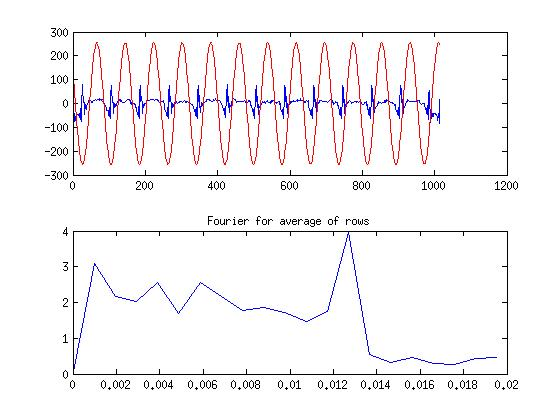
\includegraphics[width=0.8\textwidth]{process/a421a.jpg}\\
    \caption{groundtruth行平均值和其傅里叶变换\label{a421a}}
\end{figure}
\begin{figure}
    \centering
    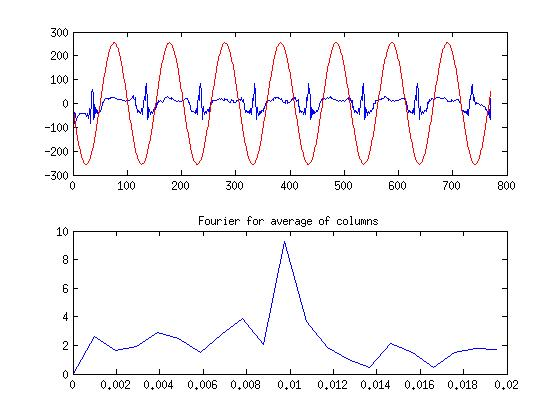
\includegraphics[width=0.8\textwidth]{process/a421b.jpg}\\
    \caption{groundtruth列平均值和其傅里叶变换\label{a421b}}
\end{figure}
\begin{figure}
    \centering
    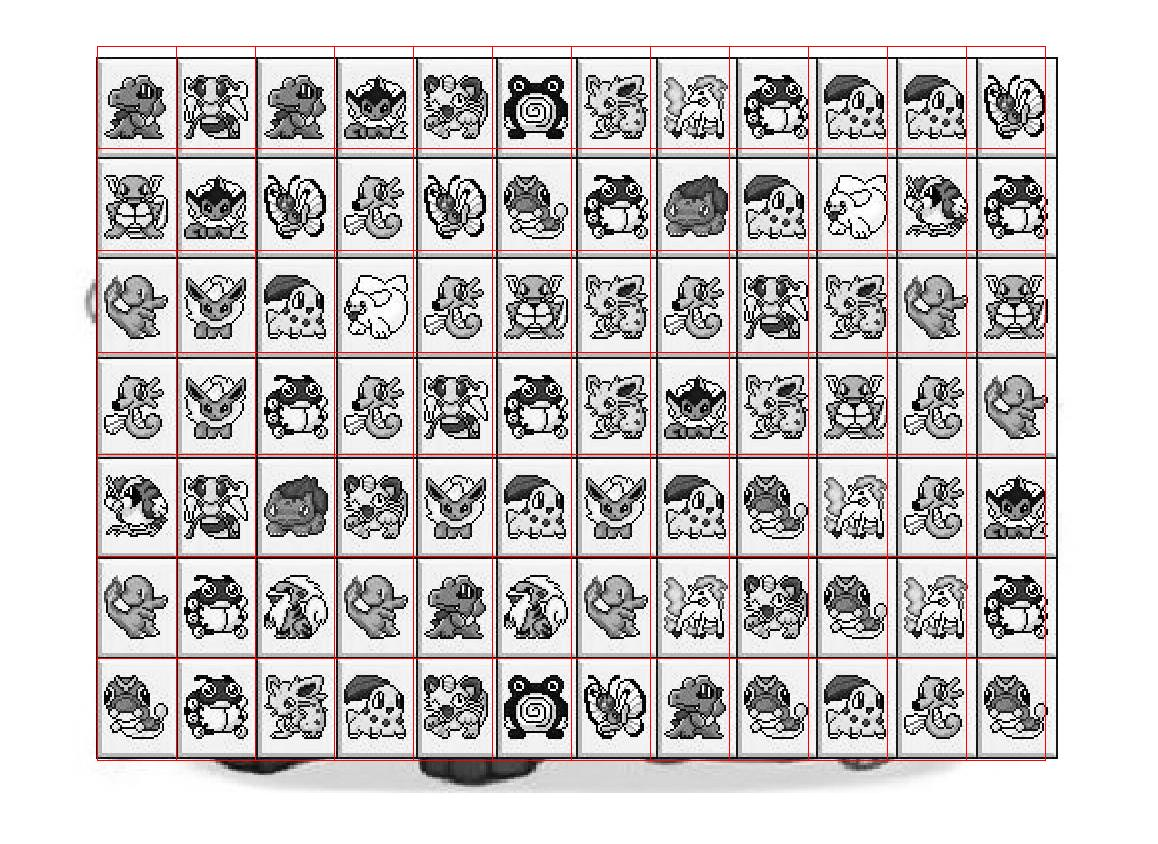
\includegraphics[width=0.8\textwidth]{process/a421c.jpg}\\
    \caption{groundtruth切割线\label{a421c}}
\end{figure}
\begin{figure}
    \centering
    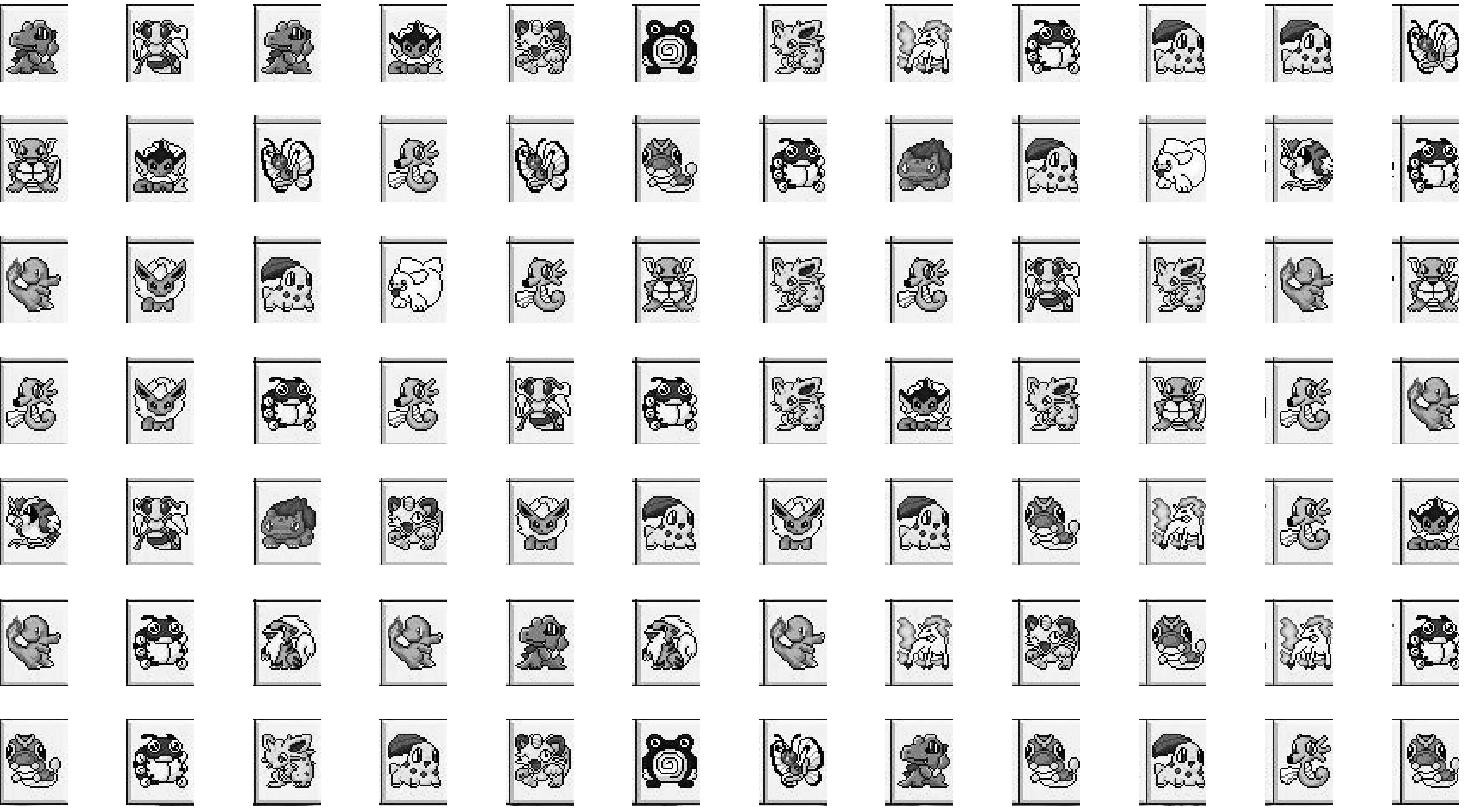
\includegraphics[width=0.8\textwidth]{process/a421d.jpg}\\
    \caption{groundtruth切割分块\label{a421d}}
\end{figure}
\subsection{对摄像头采集的图像(灰度图像)graycapture,参考第 1 题要求进行处
理。讨论:和干净图像相比,被噪声污染的图像给分块带来了什么样的困难?}
这里的处理代码和上题基本一致,模糊等问题利用高通滤波可以解决,但是graycapture这张图有明显的透视畸变,这里参照了网上的代码\footnote{手工标出图像的四个顶点\url{http://www.cnblogs.com/tiandsp/archive/2012/12/16/2820916.html}}形成了perspective这一函数进行修正。矫正后的图像如图\ref{a422a},可以看出效果不错。

最终的分割结果不错,主观上甚至好于上一题,得到的块宽54,块高68,上边沿17,左边沿23.行列的傅里叶变换分别见图\ref{a422b}和图\ref{a422c},切割线见\ref{a422d},切割后的图像见\ref{a422e}。
代码如下(a4\_2\_2.m)
\lstinputlisting[language=matlab]{process/a4_2_2.m}
perspective.m:
\lstinputlisting[language=matlab]{process/perspective.m}
\begin{figure}
    \centering
    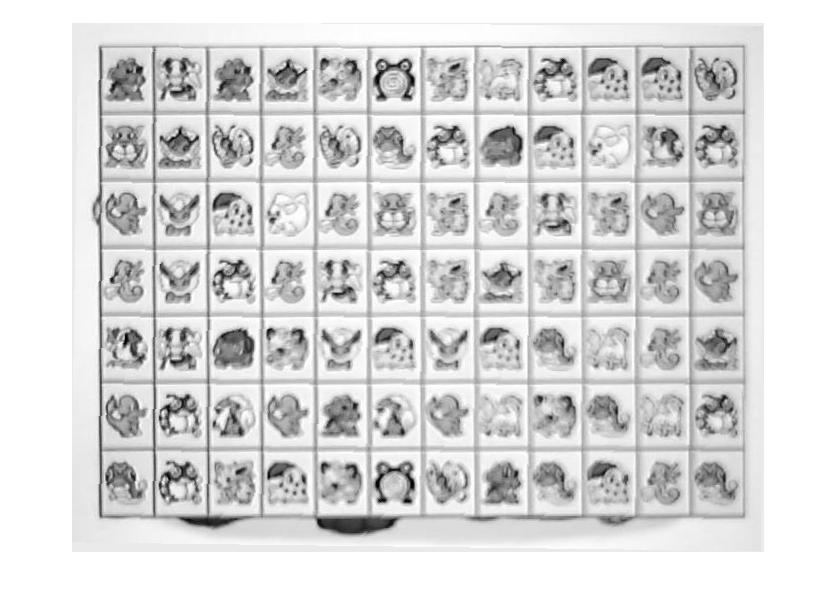
\includegraphics[width=0.8\textwidth]{process/a422a.jpg}\\
    \caption{透视矫正后的capture图像\label{a422a}}
\end{figure}

\begin{figure}
    \centering
    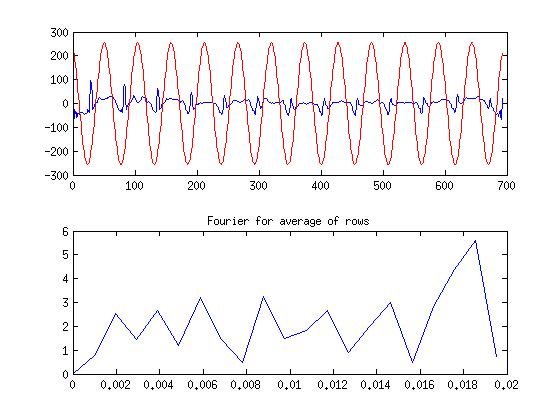
\includegraphics[width=0.8\textwidth]{process/a422b.jpg}\\
    \caption{capture行平均值和其傅里叶变换\label{a422b}}
\end{figure}
\begin{figure}
    \centering
    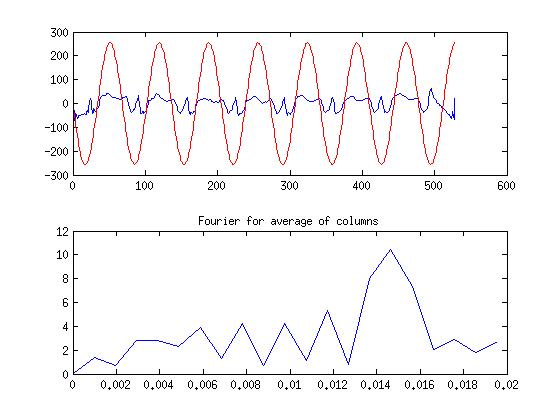
\includegraphics[width=0.8\textwidth]{process/a422c.jpg}\\
    \caption{capture列平均值和其傅里叶变换\label{a422c}}
\end{figure}
\begin{figure}
    \centering
    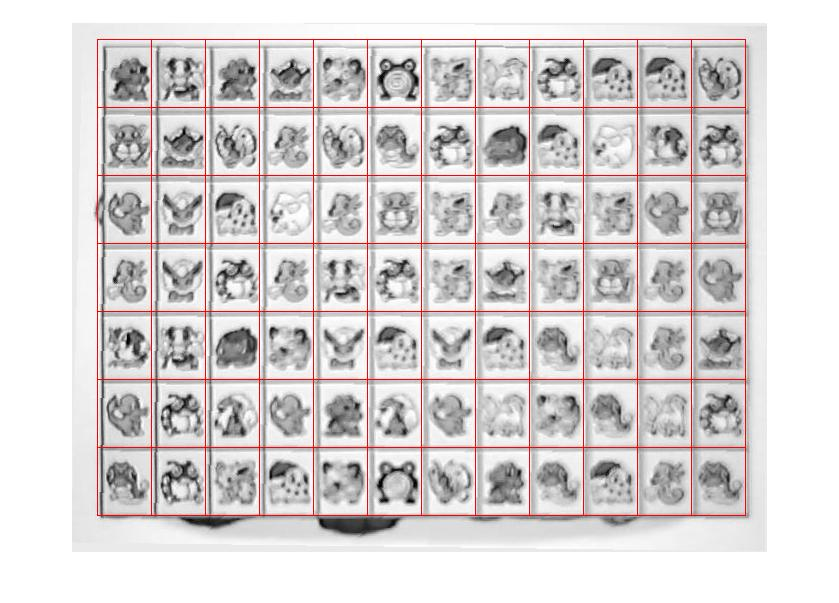
\includegraphics[width=0.8\textwidth]{process/a422d.jpg}\\
    \caption{capture切割线\label{a422d}}
\end{figure}
\begin{figure}
    \centering
    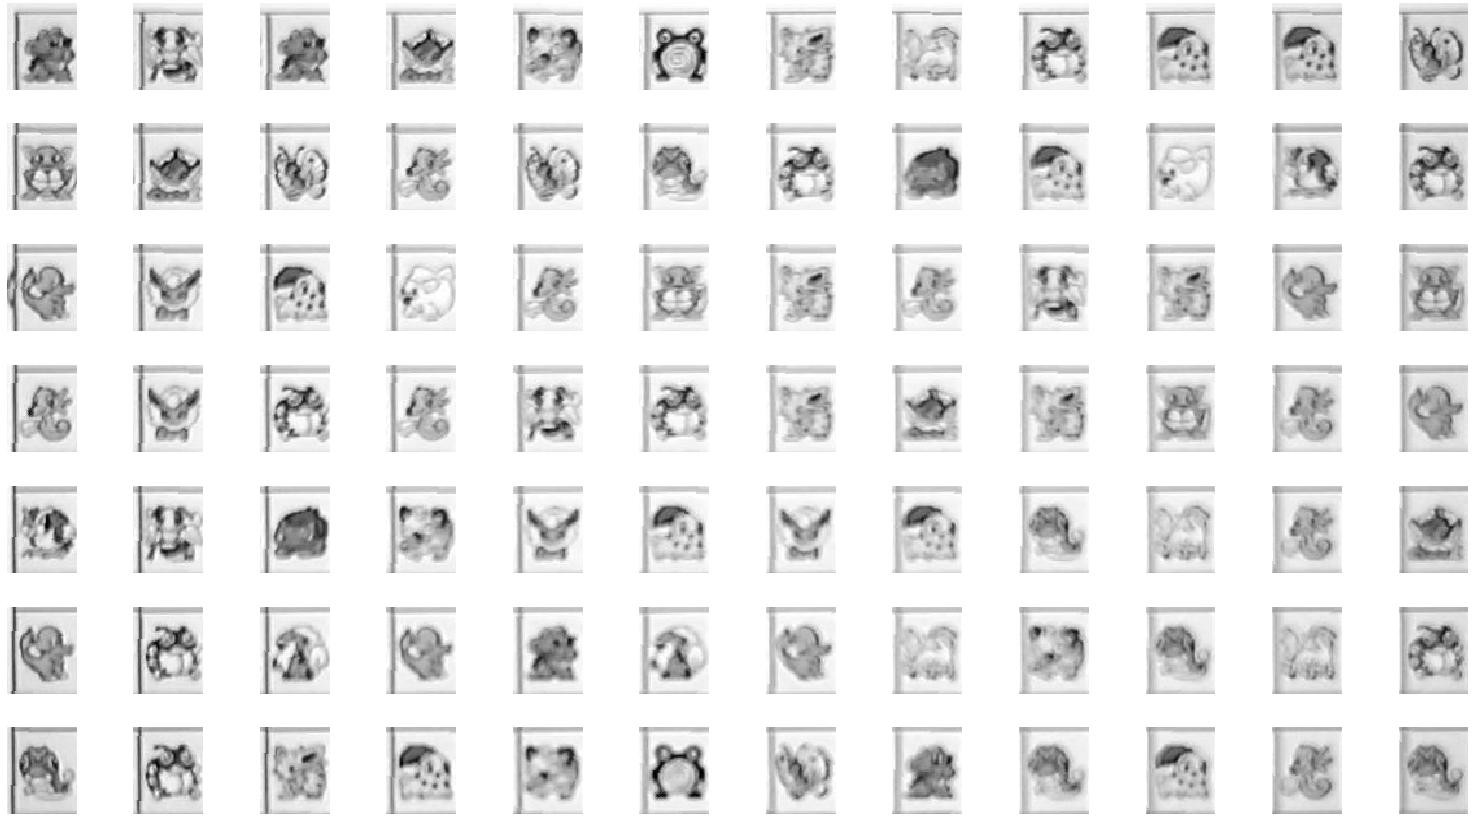
\includegraphics[width=0.8\textwidth]{process/a422e.jpg}\\
    \caption{capture切割分块\label{a422e}}
\end{figure}

\subsection{
在第 2 题基础上,计算所有图像分块的两两相似性,选出最相似的十对图
像 块 。 在 一 个 figure 中 绘 出 , 并 显 示 其 相 似 性 度 量 值 。( 建 议 先 利 用
graygroundtruth 测试代码的正确性,然后再用 graycapture 完成本题。)
}
首先利用fir1函数产生高通滤波器如图\ref{a423a},将其冲激响应旋转一周后得到图\ref{a423b},将其与各分块后的图像卷积即可得到其高通滤波后的值。

随后两两计算各个图片的内积,这里经过查询利用normxcorr2函数得到归一化的比较值。因为两个图片交换位置求相关的值有一定的差异,为了下一题好算这里取更大的那个。

这里的计算量比较大,我的笔记本大概需要运算15s左右,感觉也很难进一步压缩时间。得到图\ref{a423c}
代码如下a4\_2\_3.m
\lstinputlisting[language=matlab]{process/a4_2_3.m}
\begin{figure}
    \centering
    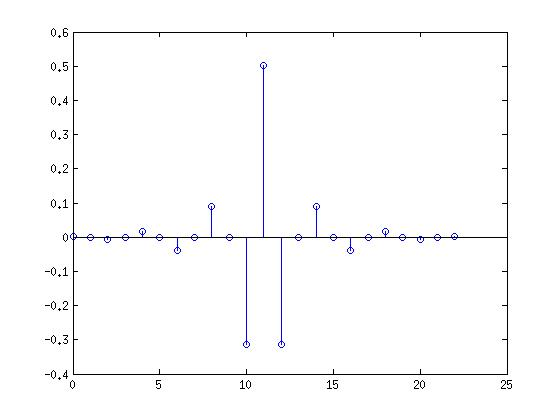
\includegraphics[width=0.8\textwidth]{process/a423a.jpg}\\
    \caption{高通滤波器的冲激响应\label{a423a}}
\end{figure}

\begin{figure}
    \centering
    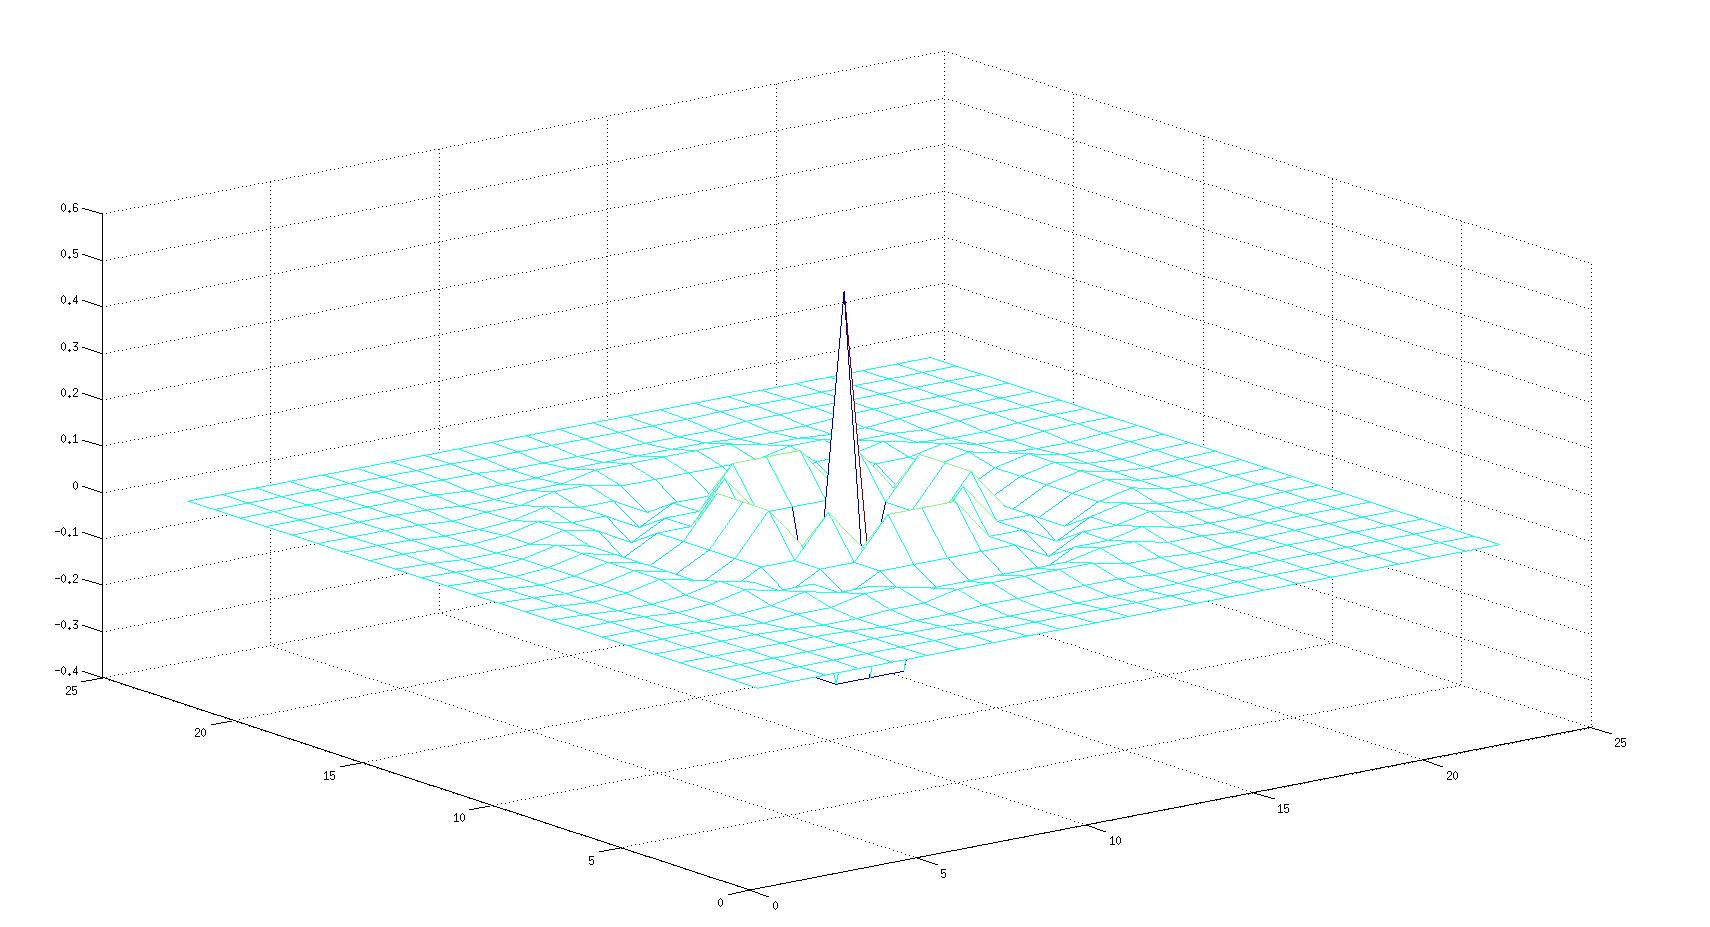
\includegraphics[width=0.8\textwidth]{process/a423b.jpg}\\
    \caption{旋转后的高通滤波器\label{a423b}}
\end{figure}
\begin{figure}
    \centering
    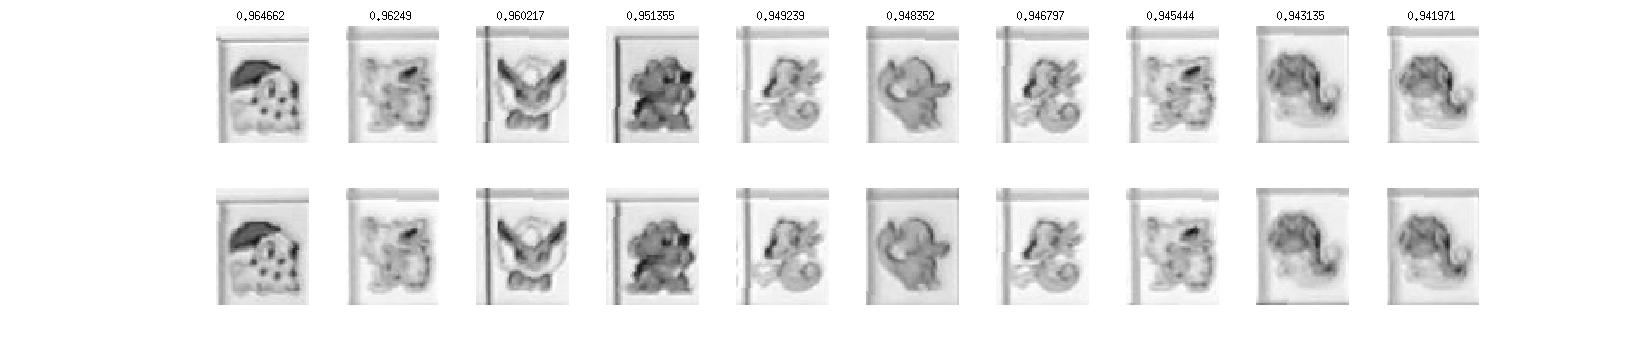
\includegraphics[width=0.8\textwidth]{process/a423c.jpg}\\
    \caption{最相近的十对\label{a423c}}
\end{figure}

\subsection{
第 3 题基础上,找出相似度最大却不是同一种精灵的十对图像块。在一个 figure 中绘出,并显示其相似性度量值。讨论:这个结果和你的主观感受
一致吗?}
挑选出来的十对图像如图\ref{a424a},可以看出,虽然人能比较容易的区分它们,但它们都是颜色比较深的图像,相似度值还是比较高的。
\begin{figure}
    \centering
    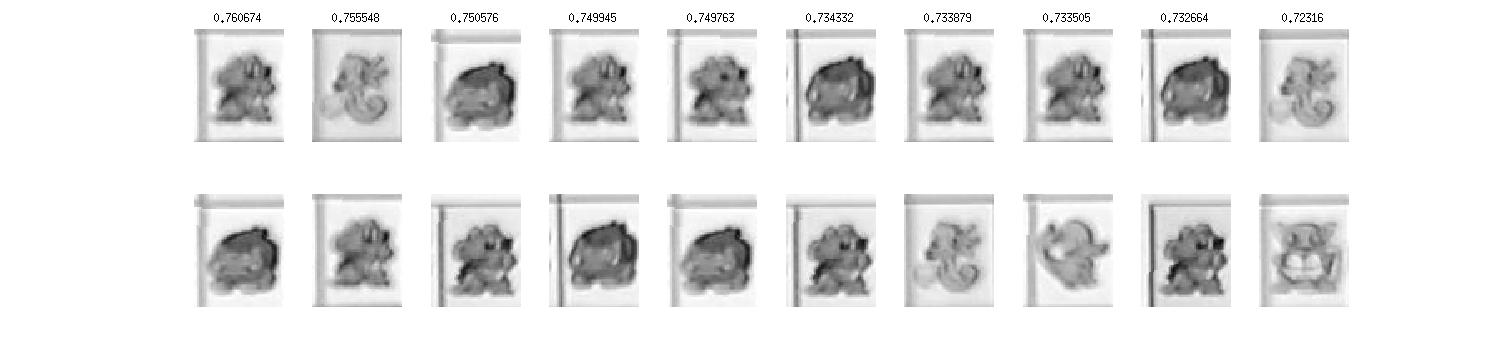
\includegraphics[width=0.8\textwidth]{process/a424a.jpg}\\
    \caption{相似度最大却不同的十对\label{a424a}}
\end{figure}
\subsection{
 在第 3 题基础上,将游戏区域映射为索引值的数组,并列出索引值和图像
分块的对照关系表。讨论:你可以将全部图像分块正确映射到其索引值吗?哪些
分块无法正确映射?为什么?
}
不得不提的是,海狮,也就是图\ref{a425}中编号15的块的两块之间相似性度量值只有0.6左右\footnote{应该是颜色太淡的原因},从上一题的结果即可看出,若直接用设定阈值的方法,这两块是无法被识别的,我开始这样试的时候也是如此。

因此我对这一方法进行了增强。这里的做法是先寻找每一个块的最相似的块,然后两两分组(此时也会得到因为两两最相似而多个块被放在一个集合里的情况)。再处理这些集合,利用阈值选择一些关系(取大于0.77,这一系数由上一问得到)把包含着一样图像的集合合并,各个集合去重后再依次给mtx的对应点赋值。

得到的矩阵如下,其中各个数字对应的图像如图\ref{a425}所示。比对后是完全正确的。
\begin{figure}
    \centering
    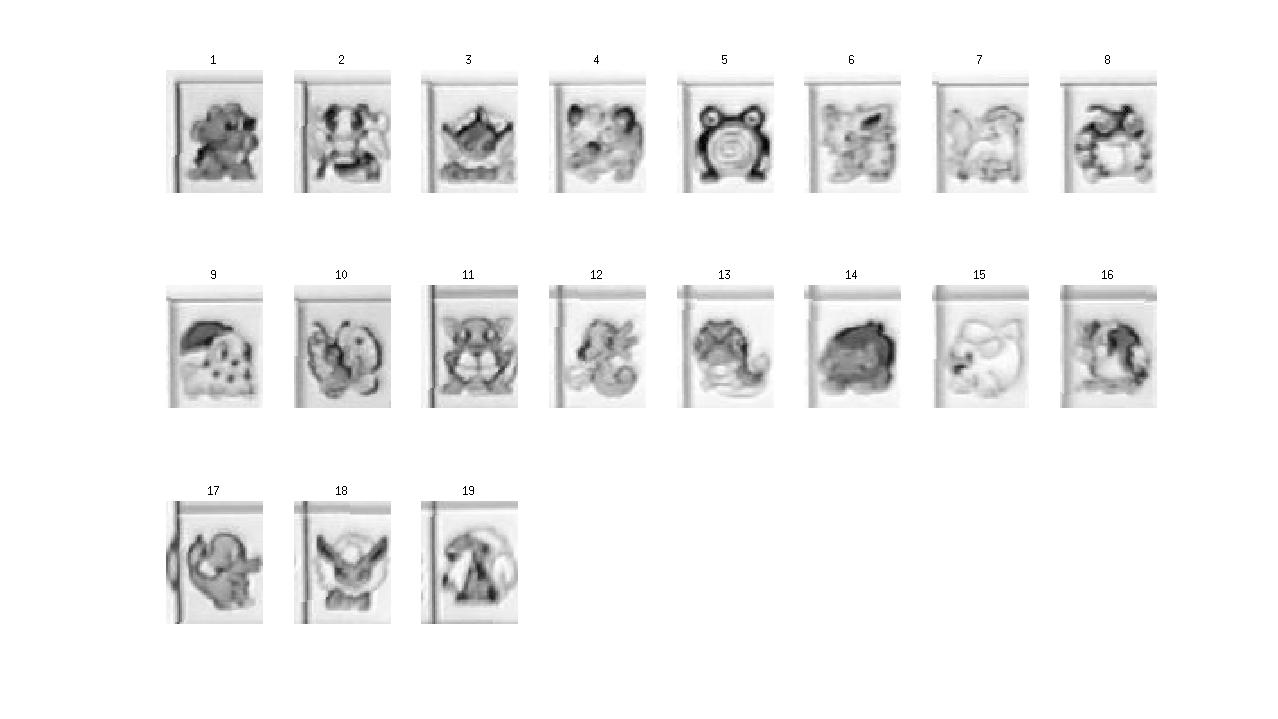
\includegraphics[width=0.8\textwidth]{process/a425.jpg}\\
    \caption{每种编号对应的图像\label{a425}}
\end{figure}
\[\begin{array}{cccccccccccc}
1&2&1&3&4&5&6&7&8&9&9&10\\
11&3&10&12&10&13&8&14&9&15&16&8\\
17&18&9&15&12&11&6&12&2&6&17&11\\
12&18&8&12&2&8&6&3&6&11&12&17\\
16&2&14&4&18&9&18&9&13&7&12&3\\
17&8&19&17&1&19&17&7&4&13&7&8\\
13&8&6&9&4&5&10&1&13&9&12&13
\end{array}\]
代码如下(a4\_2\_5.m)
\lstinputlisting[language=matlab]{process/a4_2_5.m}

\subsection{
在上述工作基础上,设计实现一个模拟的自动连连看。对摄像头采集的图
像(灰度图像)graycapture 进行分块并找出最相似的一对可消除分块后,将
这图片上两个块的位置设为黑色或其他特定颜色(即模 拟消除操作),并将图片
展示在 figure 上。然后继续找出下一对可消除的分块并模拟消除,直至消除所
有的分块或找不到可消除的分块对。设计一种方法验证并展示上述工作的正确性。
}
我的做法是没延时1.5s给被消除的一对加上标记,最终结果如图\ref{a426}

\begin{figure}
    \centering
    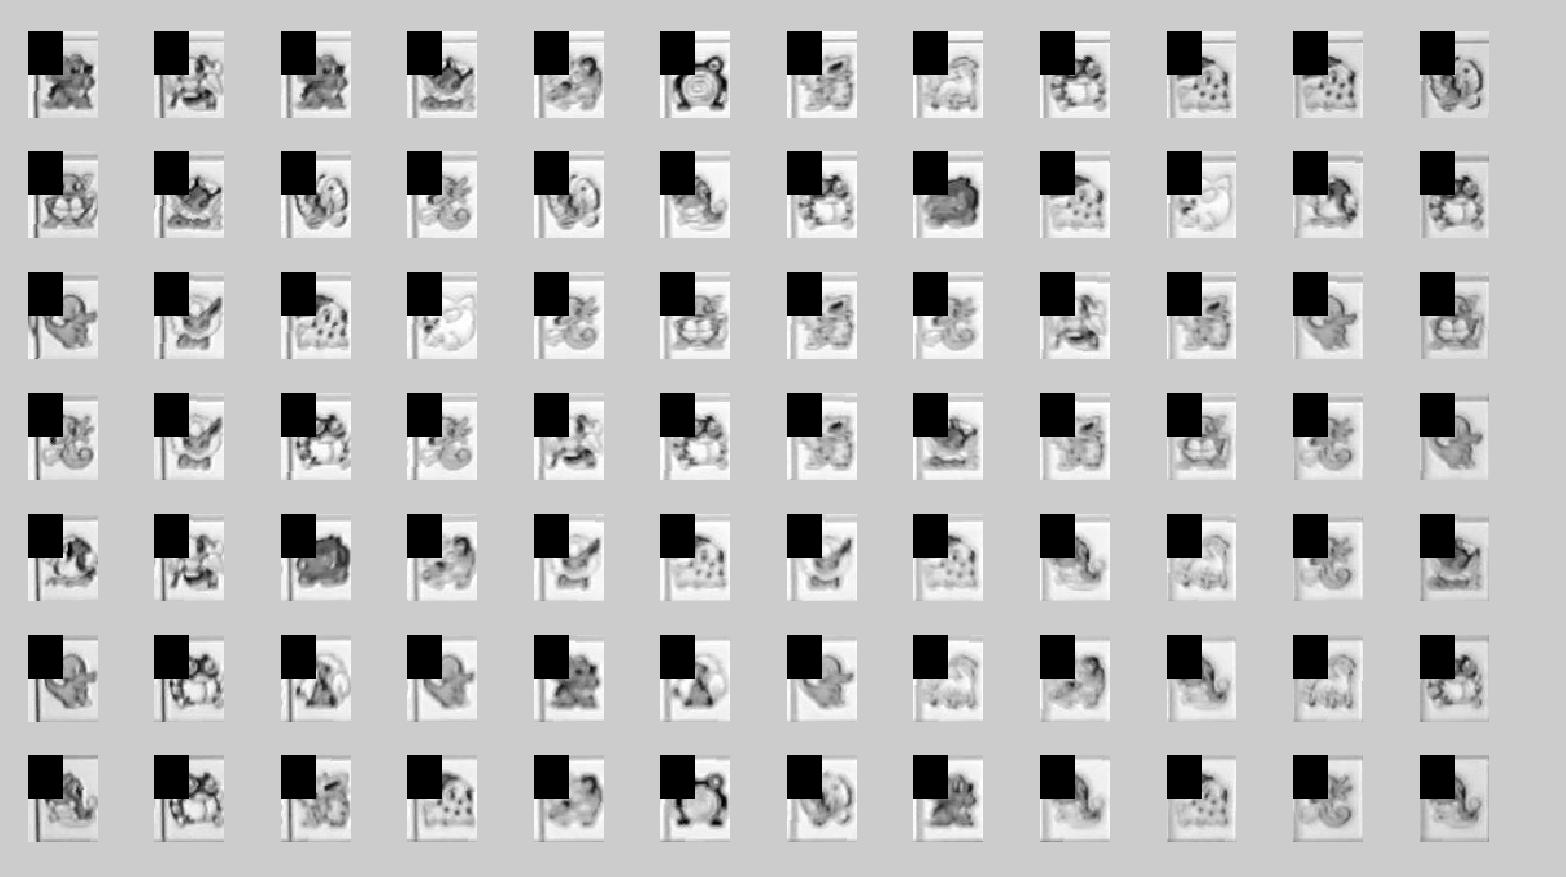
\includegraphics[width=0.8\textwidth]{process/a426.jpg}\\
    \caption{模拟连连看最终结果\label{a426}}
\end{figure}

这里通过观察消除过程可见程序是成功的,屏幕录像可以看根目录的solve.mp4文件。有趣的是,当我想调用之前的omg.m时却发现不能解出这一连连看。在调整了图像的扫描顺序后就得到了解。可见对于之前的算法,不同的扫描策略会导致有解无解的差异,但如何去覆盖所有的情况已经超出了讨论范围,这里也就不再修改。

代码如下a4\_2\_6.m
\lstinputlisting[language=matlab]{process/a4_2_6.m}

\section{实验总结}
本试验非常有趣,选取了连连看这一常见的游戏结合图像处理。

相对来说,连连看的逻辑比较好完成,而图像处理比较复杂。实验中我虽然使用了畸变矫正、高通滤波等方法,但是识别的效果依然不理想。这时只能用更强的判断算法去解决。这应该也是信号处理中经常要去面对的问题——输入信号好则算法简单但是收集难度大,输入信号差则收集难度小但算法复杂,实际的系统设计也一定是在这两者之间寻找平衡。本次实验是我对这一过程有了更深刻的理解。

除此之外,在进行映射为数组的过程中,因为matlab的二维矩阵各行必须等长,所以我不得不使用了元胞数组(cell)这一数据结构,同时还知道了fir1和normxcorr2这两个系列函数的使用,收货很大。

虽然没有进一步做的选作部分,但是我设想,彩色图像可以在三个维度上进行综合比较(平均或最大值),实际的摄像头肯定在去畸变和去噪后也是一样的处理方法,但是很难做到实时读取。
\end{document}
